\chapter{Tracking of X-Rays}
\label{c:xray.track}

\bmad can track both charged particles and X-rays. This chapter deals
with X-rays. Charged particles are handled in chapter~\sref{c:charged.track}.

%-------------------------------------------------------------------------
%-------------------------------------------------------------------------
\section{Coherent and Incoherent Photon Simulations}
\label{s:coher.incoher}

\index{coherent tracking}\index{incoherent tracking}
\bmad can track photons either \vn{coherenly} or \vn{incoherently}.
In both cases, the photon has a transverse electric field 
\Begineq
  (E_x, E_y)
\Endeq
$E_x$ and $E_y$ are complex and therefore have both amplitude and phase
information. When photons are tracked incoherently, the phase
information is not used for calculating X-ray intensities.

In addition to coherent and incoherent tracking, partially coherent
simulations can be done by using sets of photons with the photons in
any one set treated as coherent and the photons between sets being
treated as incoherent.

%-------------------------------------------------------------------------
\subsection{Incoherent Photon Tracking}
\label{s:incoher}

In a simulation with incoherent photons, some number of photons,
$N_0$, will be generated and the i\Th photon ($i = 1, \ldots, N_0)$
will have a initial ``electric field'' components $E_{x0}(i),
E_{y0}(i)$ assigned to it. The field amplitude $E_0$ will be
$\sqrt{E_{x0}^2 + E_{y0}^2}$.

At some an observation point, the power $S$ per unit area falling on
some small area $dA$ due to either $x$ or $y$ component of the
electric field is
\Begineq
  S_{x,y} = \frac{\alpha_p}{N_0 \, dA} \, \sum_{j \in \text{hits}} E_{x,y}^2(j)
  \label{panda1}
\Endeq
where $\alpha_p$ is a constant that can be chosen to fit the
simulation against experimental results, and the sum is over photons
who intersect the area. The factors of $N_0$ and $dA$ in the above
equation make, within statistical flucuations, $S$ independent of
$N_0$ and, for $dA$ small enough, $S$ will be independent of $dA$ as
it should be. The total power is just $S_x + S_y$.

When traveling through vacuum, the electric field of a photon is a
constant.  As an example, consider a point source raidiating uniformly
in $4\pi$ solid angle with each photon having the same initial field
$E_0$. An observation area $dA$ situated a distance $R$ from the
source will intercept $N_0 \, dA / 4 \, \pi \, R^2$ photons which
gives a power of
\Begineq
  S_w = \frac{\alpha_p \, E_0^2}{4 \, \pi \, R^2}
\Endeq
which falls off as $1/R^2$ as expected.

At some places the light may be split into various ``channels''. An
example is Laue diffraction where X-rays can excite the $\alpha$ and
$\beta$ branches of the dispersion surface. Or a partially silvered
mirror where some of the light is reflected and some is transmitted.
In such a case, the probability $P_i$ of a photon traveling down the
$i$\Th channel is
\Begineq
  P_i \, \what E_i^2 = \frac{S_i}{S_0}
  \label{rpss1}
\Endeq
where $S_i$ is the power flowing into channel $i$, $S_0$ is the power
flowing into the junction, and $\what E_i = E_i / E_0$ is the ratio of
the electric field amplitudes of any photon just before and just after being
shunted into the $i$\Th channel. The probabilities must be properly
normalized
\Begineq
  \sum P_i = 1
  \label{p1}
\Endeq

If the ratio of the electric field of any photon just before and just
after being shunted into the $i$\Th channel is not a constant, than
$\what E_i$ must be adjusted so that $\what E_i^2$ is equal to the average of
$\what E_i^2(j)$ for all photons $j$ channeled into channel $i$.

As long as \Eqs{rpss1} and \eq{p1} are satisfied, the choice of the
$P_i$, and $\what E_i$ are arbitrary. This freedom allows simulation to be
optimized for efficiency. For example, In an actual experiment much of
the light can be lost never to reach a detector and be counted. To
decrease the simulation time, simulated photons may be limited to be
generated with a direction to be within some solid angle $\Omega_1$ if
photons with a direction outside this solid angle will not contribute
to the simulation results. In this case, there are two channels.
Channel 1 consists of all photons whose direction is within
$\Omega_1$ and channel 2 is all the other photons. To limit the
photons to channel 1, $P_1$ is taken to be 1 and $P_2$ is taken to be
0. Additionaly, if the light, say, is being generated isotropically
from a surface into a $\Omega_0 = 2 \, \pi$ solid angle then
\Begineq
  \what E_1 = \sqrt{\frac{\Omega_1}{\Omega_0}}
  \label{roo}
\Endeq
$\what E_2$ is infinite here but since no photons are generated in channel 2
this is not a problem.

%-------------------------------------------------------------------------
\subsection{Coherent Photon Tracking}
\index{ss:coher}

In a simulation with coherent photons, some number of photons,
$N_0$, will be generated and the i\Th photon ($i = 1, \ldots, N_0)$
will have an initial electric field $E_{x0}(i), E_{y0}(i)$ assigned to
it. These quantities will be complex.

At some an observation point, the field $E$ at
some small area $dA$ due to either $x$ or $y$ component of the
electric field is
\Begineq
  E = \frac{\alpha_p}{N_0 \, dA} \, \sum_{j \in \text{hits}} E(j)
  \label{panda2}
\Endeq
where $\alpha_p$ is a constant that can be chosen to fit the
simulation against experimental results, and the sum is over photons
who intersect the area. In the above equation $E(j)$ is either the $x$
or $y$ component of the electric field as is appropriate. The factors
of $N_0$ and $dA$ in the above equation make, within statistical
flucuations, $E$ independent of $N_0$ and, for $dA$ small enough, $E$
will be independent of $dA$ as it should be.

When traveling through a a vacuum, the photons travel ballistically in
straight lines. This is justified by using the stationary phase
approximation with Kirchhoff's integral. the electric field of a
photon varies with the propagation length. There is nothing physical
in this and is just a way to make the bookkeeping come out
correctly. As an example, consider a point source raidiating uniformly
in $4\pi$ solid angle with each photon having the same initial field
component (either $x$ or $y$) $E_1$.  An observation area $dA$
situated a distance $R$ from the source will intercept $N_0 \, dA / 4
\, \pi \, R^2$ photons and each photon will have a field of $E_1 \, R
\, \exp(i \, k \, R)$ where $k$ is the photon wave number (all photons
must have the same $k$ to be coherent). This gives an electric field
at the observation point of
\Begineq
  E = \frac{\alpha_p \, E_1 \, \exp(i \, k \, R)}{4 \, \pi \, R}
\Endeq
which falls off as $1/R$ as expected.

At a \vn{diffraction_plate} element where diffraction effects are to
be simulated, the following procedure is used:
  \begin{enumerate}
  \item
The electric field components are multiplied by the propagation length $L$:
\Begineq
  E \rightarrow E \, L
\Endeq
The propagation length is reset to zero so that the at the next point
where the propagation length is factored into the electric field the
propagation length will be the length starting at the aperture.
  \item
Depending upon the program, the photon is is either given a random
direction over $2 \, \pi$ solid angle or the photon's direction
is restricted to be within some solid angle choosen to increase
the probability that the photon will make it through some downstream aperture.

If the photon is restricted to some aperture dependent solid angle of area $\Omega$,
the photon's electric field is scalled by
\Begineq
  E \rightarrow E \, \frac{\Omega}{4 \, \pi}
  \label{eeo4p}
\Endeq

  \item
The electric field components are scaled by
\Begineq
  E \rightarrow E \, \frac{k}{4 \, \pi \, i} \, (\cos\theta_1 + \cos\theta_2)
  \label{eek4p}
\Endeq
where $\theta_1$ and $\theta_2$ are the dirction cosines of the
incoming and outgoing directions of the photon with respect to the
longitudinal reference axis.
  \end{enumerate}
This algorithm is designed so that the resulting fields at points
downstream from the aperture as computed from a simulation will, to
within statistical errors, be the same as one would get using
Kirchoff's integral. That is, the simulation is constructed to be a
Monte Carlo integration of Kirchhoff's integral.

What is, and what is not considered a place where there are
diffraction effects is dependent upon the problem. For example, there
are diffraction effects associated with light reflecting from a mirror
(or any other object) of finite size. If these effects are important
to the experiment, then a procedure similar to the one above must be
followed. 

At places where there are no diffraction effects a simulation can
treat the photons ballistically or can use the aperture procedure
outlined above. While in theory it is possible to choose what to do, in
practice the aperture procedure increases the number of photons that
must be tracked for a given resolution. Thus, from a practical standpoint
the ballistic alternative should always be used.

As explaned in \sref{s:incoher}, at some places the light may be split
into various ``channels''. With coherent photons, the analog to \Eq{rpss1} is
\Begineq
  P_i \, \what E_i = \frac{E_i}{E_0}
  \label{rpss2}
\Endeq
where here $\what E_i$ can be complex to take into account phase shifts.
The same considerations about choosing the $P_i$ and $\what E_i$ apply to
coherent photons as incoherent photons. In particular, $\what E_1$ for the
case of isotropic emission from a surface as in the equample in
\sref{s:incoher} (cf. \Eq{roo}) is
\Begineq
  \what E_1 = \frac{\Omega_1}{\Omega_0}
\Endeq

%-------------------------------------------------------------------------
\subsection{Parially Coherent Photon Simulations}

When there is partial coherence the photons must be divided into
sets. All of the photons of a given set are considered coherent while
the photons of different sets are treated incoherently.

The procedure is to track all the photons of one set coherently and
calculate the field using equation \Eq{panda2}. The fields of
different sets are then combined to calculate a power using
\Eq{panda1}.

%-------------------------------------------------------------------------
%-------------------------------------------------------------------------
\section{Element Coordinate System}
\label{s:photon.ele.coords}

\index{element coordinates}
The general procedure for tracking through an element makes use of
\vn{element reference} coordinates (also called just \vn{element}
coordinates). Without any offsets, pitches or tilt (\sref{s:offset}), henceforth
called ``misalignments'', the \vn{element} coordinates are the same
as the \vn{laboratory reference} coordinates (or simply \vn{laboratory}
coordinates) (\sref{s:ref}). The \vn{element} coordinates stay fixed
relative to the element. Therefore, if the element is misaligned, the
\vn{element coordinates} will follow as the element shifts in the
laboratory frame as shown in \fig{f:ele.coord}.

\index{crystal}\index{mirror}\index{multilayer_mirror}
For \vn{crystal} (\sref{s:crystal}), \vn{mirror} (\sref{s:mirror}), and \vn{multilayer_mirror}
(\sref{s:multilayer}) elements, the ``kinked'' reference trajectory through the element complicates
the calculation. For these elements, there are three coordinate systems attached to the element as
shown in \fig{f:photon.ele.coords}. Besides the \vn{element entrance} and \vn{element exit}
coordinates, there are \vn{element surface} coordinates with $z$ perpendicular to the surface
pointing inward.

Tracking a particle through an element is therefore a three
step transformation:
\begin{enumerate}[itemsep=-0.1ex, topsep=-0.4ex]
\item
At the entrance end of the element, transform from the laboratory
reference coordinates to the element's \vn{entrance} or \vn{surface}
coordinates.
\item
Track through the element ignoring any misalignments.
\item
At the exit end of the element, transform from the element coordinates
to the \vn{laboratory} \vn{exit} coordinates.
\end{enumerate}


%-------------------------------------------------------------------------

\begin{figure}[tb]
  \centering
  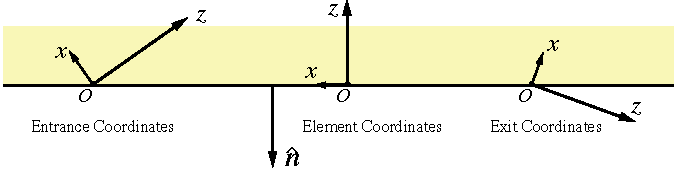
\includegraphics[width=5in]{photon-ele-coords.pdf}
  \caption[Crystal, Mirror, and Multilayer_Mirror Element Coordinates.]
{The three element coordinate systems for \vn{crystal} (Bragg
configuration), \vn{mirror}, and \vn{multilayer_mirror} elements.  The
origin $\Bf O$ of all three are the same but are shown spread out for
clarity.  $\bfhat n$ is the normal to the element surface.}
  \label{f:photon.ele.coords}.
\end{figure}

%-------------------------------------------------------------------------
\subsection{Transform from Laboratory Entrance to Element Coordinates}

For elements that have a reference orbit kink
(\sref{s:photon.ele.coords}), the element coordinates here are the
\vn{surface} coordinates. Otherwise the element coordinates are
the entrance coordinates.

  \begin{enumerate}
  \item
Apply offsets, pitches and tilt using the formulas in
\sref{s:pos.trans} along with \Eqs{wws}, and \eq{swww}.
  \item
Apply the \vn{tilt} to the electric field (\Eq{ertee}).
  \item
For \vn{crystal}, \vn{mirror}, and \vn{multilayer_mirror} elements
rotate to element surface coordinates.
 \item
Transform the photon's position as if in a drift by a distance $-z$
where $z$ is the photon's longitudinal coordinate. That is, $z$ will
be zero at the end of the transform to element coordinates (remember
that $z$ is the distance from the start of the element
(\sref{s:photon.phase.space})).

\end{enumerate}

%-------------------------------------------------------------------------
\subsection{Transform from Element Exit to Laboratory Coordinate}

The back transformation from element to laboratory coordinates is
accomplished by the transformation
  \begin{enumerate}
  \item
For \vn{crystal}, \vn{mirror}, and \vn{multilayer_mirror} elements
rotate to element from element surface coordinates to element exit coordinates
  \item
Apply the reverse \vn{tilt} to the electric field (\Eq{ertee}).
  \item
Apply reverse offsets, pitches and tilt using the formulas in
\sref{s:pos.trans} along with \Eqs{wws}, and \eq{swww}.
  \end{enumerate}

%-------------------------------------------------------------------------
%-------------------------------------------------------------------------
\section[Mirror and Crystal Element Transformation]
{Transformation for Mirror and Crystal Elements Between 
Laboratory and Element Coordinates}
\label{s:photon.lab.ele}

\index{mirror}\index{crystal}

%-------------------------------------------------------------------------
\subsection{Transformation from Laboratory to Element Coordinates}
\label{s:crystal.trans.le}

\index{z_offset_tot}
With photons, the intensities must also be transformed.
The transformation from the entrance laboratory coordinates to
the entrance element coordinates is:
\begin{enumerate}
\item
Track as in a drift a distance \vn{z_offset_tot}.
\item
\index{x_offset}\index{x_pitch}\index{y_offset}\index{y_pitch}
Apply offsets and pitches: The effective ``length'' of the element is
zero (\sref{s:mirror.coords}) so the origin of the element coordinates
is the same point around which the element is pitched so
\begin{align}
  x_1    &= x_0 - x_{\text{off}} \CRNO
  p_{x1} &= p_{x0} - (1 + p_{z0}) \, x'_{pitch} \CRNO
  y_1    &= y_0 - y_{\text{off}} \\
  p_{y1} &= p_{x0} - (1 + p_{z0}) \, y'_{pitch} \CRNO
  z_1    &= z_0 + x'_{pitch} \, x_1 + y'_{pitch} \, y_1 \nonumber
\end{align}
where $x_{\text{off}} \equiv \vn{x_offset}$, $x'_{pitch} \equiv \vn{x_pitch}$, etc.
\item
Apply \vn{ref_tilt} and \vn{tilt}:
\begin{align}
  \begin{pmatrix} x_2 \\ y_2 \end{pmatrix} &=
    \bfR (\theta_{tot}) \,   
  \begin{pmatrix} x_1 \\ y_1 \end{pmatrix} \CRNO
  \begin{pmatrix} p_{x2} \\ p_{y2} \end{pmatrix} &=
    \bfR (\theta_{tot}) \, 
  \begin{pmatrix} p_{x1} \\ p_{y1} \end{pmatrix} \label{xyrtxy} \\ 
  \begin{pmatrix} \bfE_{x2} \\ \bfE_{y2} \end{pmatrix} &=
    \bfR (\theta_{tot}) \,   \begin{pmatrix} \bfE_{x1} \\ \bfE_{y1} \end{pmatrix} \nonumber
\end{align}
where $\bfE$ is shorthand notation for
\Begineq
  \bfE \equiv E \, e^{i \, \phi}
\Endeq
with $E$ being the field intensity and $\phi$ being the field phase angle.
In the above equations $\bfR$ is the rotation matrix
\Begineq
  \bfR(\theta) = \begin{pmatrix} \cos\theta & \sin\theta \\ -\sin\theta & \cos\theta \end{pmatrix}
\Endeq
\index{tilt}\index{ref_tilt}\index{tilt_corr}
with $\theta_{tot}$ being 
\Begineq
  \theta_{tot}  = 
  \begin{cases}
    \vn{ref_tilt} + \vn{tilt} + \vn{tilt_corr} & \vn{for crystal elements} \\
    \vn{ref_tilt} + \vn{tilt} & \vn{for mirror elements}
  \end{cases}
  \label{tttt}
\Endeq
The \vn{tilt_corr} correction is explained in \sref{s:crystal.trans}.
\end{enumerate}

%-------------------------------------------------------------------------
\subsection{Transformation from Element to Laboratory Coordinates}
\label{s:crystal.trans.el}

The back transformation from exit element coordinates to exit
laboratory coordinates is accomplished by the transformation
  \begin{enumerate}
  \item
Apply \vn{ref_tilt} and \vn{tilt}: \vn{ref_tilt} rotates the exit
laboratory coordinates with respect to the exit element coordinates in
the same way \vn{ref_tilt} rotates the entrance laboratory coordinates
with respect to the entrance element coordinates. The forward and back
transformations are thus just inverses of each other.  With
\vn{tilt}, this is not true. \vn{tilt}, unlike \vn{ref_tilt}, does
not rotate the output laboratory coordinates.  There is the further
complication in that \vn{tilt} is a rotation about the {\em
entrance} laboratory coordinates. The first step is to express
\vn{tilt} with respect to the exit coordinates. This is done with
the help of the $\bfS$ matrix of \Eq{ustt} with $\alpha_t$ given by
\Eq{agg}. The effect of the \vn{tilt} can be modeled as a rotation
vector $\Bf e_{in}$ in the entrance laboratory coordinates pointing
along the $z$-axis
\Begineq
 \Bf e_{in} = (0, 0, \text{tilt})
\Endeq
In the exit laboratory coordinates, the vector $\Bf e_{out}$ is
\Begineq
  \Bf e_{out} = \bfS \, \Bf e_{in}
\Endeq
The $z$ component of $\Bf e_{out}$ combines with \vn{ref_tilt} to give
the transformation
\begin{align}
  \begin{pmatrix} x_2 \\ y_2 \end{pmatrix} &=
    \bfR (-\theta_{t}) \,   \begin{pmatrix} x_1 \\ y_1 \end{pmatrix} \CRNO
  \begin{pmatrix} p_{x2} \\ p_{y2} \end{pmatrix} &=
    \bfR (-\theta_{t}) \,   \begin{pmatrix} p_{x1} \\ p_{y1} \end{pmatrix} \\
  \begin{pmatrix} \bfE_{x2} \\ \bfE_{y2} \end{pmatrix} &=
    \bfR (-\theta_{t}) \,   \begin{pmatrix} \bfE_{x1} \\ \bfE_{y1} \end{pmatrix} \nonumber
\end{align}
where $\theta_t$ is $\text{ref_tilt} + \Bf e_{out,z}$. The $x$ and $y$ components
of $\Bf e_{out}$ give rotations around the $x$ and $y$ axes
\begin{align}
  p_{x3} &= p_{x2} - \Bf e_{out,y} \CRNO
  p_{y3} &= p_{y2} + \Bf e_{out,x} \\
  z_3    &= z_2 + x_2 \, \Bf e_{out,y} - y_2 \, \Bf e_{out,x}
\end{align}
  \item
Apply pitches: Since pitches are defined with
respect to the entrance laboratory coordinates, they have to be
translated to the exit laboratory coordinates
\Begineq
  \bfP_{out} = \bfS \, \bfP_{in}
\Endeq
where $\bfP_{in} = (x'_{pitch}, y'_{pitch}, 0)$ is the pitch vector in
the entrance laboratory frame and $\bfP_{out}$ is the vector in the exit
laboratory frame. The transformation is then
\begin{align}
  p_{x4} &= p_{x3} - \bfP_{out,y} \CRNO
  p_{y4} &= p_{y3} + \bfP_{out,x} \\
  z_4    &= z_3 + x_3 \, \bfP_{out,y} - y_3 \, \bfP_{out,x}
\end{align}
  \item
Apply offsets: Again, offsets are defined with respect to the
entrance laboratory coordinates. Like pitches, the translation is
\Begineq
  \bfO_{out} = \bfS \, \bfO_{in}
\Endeq
where $\bfO_{in} = (x_{\text{off}}, y_{\text{off}}, s_{\text{off}})$ is the offset in the
entrance laboratory frame. The transformation is
\begin{align}
  x_5 &= x_4 + \bfO_{out,x} - p_{x4} \, \bfO_{out,z} \CRNO
  y_5 &= y_4 + \bfO_{out,y} - p_{y4} \, \bfO_{out,z} \\
  z_5 &= z_4 + \bfO_{out,z} 
\end{align}
  \end{enumerate}

%-------------------------------------------------------------------------

\begin{figure}[tb]
  \centering
  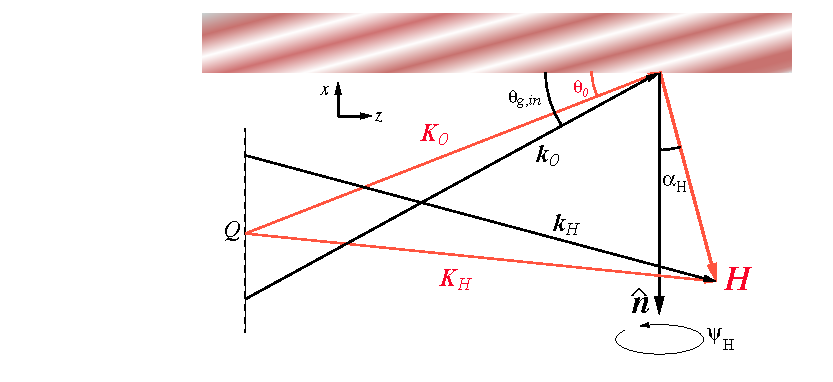
\includegraphics[width=5in]{crystal-diffraction.pdf}
  \caption[Reference trajectory reciprocal space diagram for crystal diffraction.]
{Reference trajectory reciprocal space diagram for for A) Bragg
diffraction and B) Laue diffraction. The bar over the vectors
indicates that they refer to the reference trajectory. The $x$-$z$
coordinates shown are the element surface coordinates. All points in the
diagram are in the plane of the paper except for the tip of $\bfH$.
$\bfKbar_{0}$, and $\bfKbar_{H}$ are the wave vectors inside the
crystal and $\bfkbar_{0}$ and $\bfkbar_{H}$ are the wave vectors
outside the crystal. The reference photon traveling along the
reference trajectory has $\bfKbar_0$ and $\bfKbar_H$ originating at
the $Q$ point. For Laue diffraction, the crystal faces are assumed
parallel.  For Bragg diffraction the crystal normal is in the $-\bfhat
x$ direction while for Laue diffraction the crystal normal is in the
$-\bfhat z$ direction
  }
  \label{f:crystal.diffraction}
\end{figure}

%-------------------------------------------------------------------------
%-------------------------------------------------------------------------
\section{Crystal Element Tracking}
\label{s:crystal.tracking}

\textit{\large [Crystal tracking developed by Jing Yee Chee, Ken Finkelstein, and David Sagan]}

Crystal diffraction is modeled using dynamical diffraction theory. The
notation here follows Batterman and Cole\cite{b:batterman}.  The
problem can be divided up into two parts. First the reference
trajectory must be calculated. This means calculating the incoming
grazing angle $\theta_{B,in}$ and outgoing grazing angle
$\theta_{B,out}$ as well as calculating the transformations between
the various coordinate systems. This is done in \sref{s:crystal.ref},
\sref{s:crystal.trans}, and \sref{s:laue.ref}.  The second part
is the actual tracking of the photon and this is covered in
\sref{s:bragg.track} \sref{s:coherent.laue} and \sref{s:incoherent.laue}.

%-------------------------------------------------------------------------
\subsection{Calculation of Entrance and Exit Bragg Angles}
\label{s:crystal.ref}

\fig{f:crystal.diffraction} shows the geometry of the
problem. The bar over the vectors indicates that they refer to the
reference trajectory. The reference trajectory is calculated such that
the reference photon will be in the center of the Darwin curve. That
is, the internal wave vectors $\bfKbar_0$ and $\bfKbar_H$ originate
from the $Q$ point (See \cite{b:batterman} Figs.~8 and 29).

The external wave vectors $\bf k_0$, and $\bf k_H$ and the internal wave vectors
have magnitude
\begin{align}
  |\bf k_0| &= |\bf k_H| = \frac{1}{\lambda} 
  \label{kk1l1} \\
  |\bfKbar_0| &= |\bfKbar_H| = \frac{1 - \delta}{\lambda}
  \label{kk1l2}
\end{align}
where $\lambda$ is the wavelength, and $\delta$ is
\Begineq
  \delta = \frac{\lambda^2 r_e}{2 \, \pi \, V} \, F_0' = \frac{\Gamma}{2} \, F_0'
  = \frac{1}{2} \, \Gamma \, F_0'
\Endeq
with $r_e$ being the classical electron radius, $V$ the unit cell
volume, and $F_0'$ is the real part of the $F_0$ structure factor. 

In element surface coordinates (which will be the coordinate system used
henceforth), $\bfkbar_0$ lies in the $x$-$z$ plane. $\bfKbar_0$ is
related to $\bfkbar_0$ via Batterman Eq.~(25)
\Begineq
  \bfK_0 = \bfk_0 + q_0 \, \bfhat n
  \label{kkqn1}
\Endeq
where the value of $q_0$ is to be determined. Here, and in equations
below, if the equation is true in general, and not just for the
reference trajectory, the bar superscript is dropped.

Since $\bfhat n$ is in the $-\bfhat x$ direction, $\bfKbar_0$ is also
in the $x$-$z$ plane. Thus $\bfkbar_0$ and $\bfKbar_0$ can be written
in the form
\begin{alignat}{3}
  \bfkbar_0 &= \frac{1}{\lambda} \, 
    \begin{pmatrix}
    -\cos\theta_{B,in} \\
    0 \\
    \sin\theta_{B,in}
    \end{pmatrix}
  \; , & \qquad
  \bfKbar_0 &= \frac{1 - \delta}{\lambda} \, 
    \begin{pmatrix}
    -\cos\theta_0 \\
    0 \\
    \sin\theta_0
    \end{pmatrix}
  & \qquad &\text{[Bragg]} \CRNO
  \bfkbar_0 &= \frac{1}{\lambda} \, 
    \begin{pmatrix}
    \sin\theta_{B,in} \\
    0 \\
    \cos\theta_{B,in}
    \end{pmatrix}
  \; , & \qquad
  \bfKbar_0 &= \frac{1 - \delta}{\lambda} \, 
    \begin{pmatrix}
    \sin\theta_0 \\
    0 \\
    \cos\theta_0
    \end{pmatrix}
  &\qquad & \text{[Laue]} 
  \label{k1lst}
\end{alignat}
Where, as shown in \fig{f:crystal.diffraction}, $\theta_{B,in}$, and
$\theta_0$ are the angles of $\bfkbar_0$ and $\bfKbar_0$ with respect
to the $x$-axis for Bragg reflections and with respect to the $z$-axis
for Laue reflection. 

$\alpha_H$ (\vn{alpha_angle}) is the angle that $\bfH$ makes with
respect to the $-\bfhat z$ axis and $\psi_H$ (\vn{psi_angle}) is the
rotation of $\bfH$ around the $-\bfhat z$ axis such that for $\psi_H =
0$, $\bfH$ is in the $x$-$z$ plane and oriented as shown in
\fig{f:crystal.diffraction}. Thus
\Begineq
  \bfH 
  \equiv \frac{1}{d} \, \bfhat{H} 
  = \frac{1}{d}
    \begin{pmatrix} 
       -\sin \alpha_H \, \cos \psi_H \\ \sin \alpha_H \, \sin \psi_H \\ -\cos \alpha_H
    \end{pmatrix}
  \label{h1daa}
\Endeq
where $\bfhat{H}$ is $\bfH$ normalized to 1. $\alpha_H$ is determined
via the setting of \vn{b_param} and via \Eq{batat}.

The vectors $\bfK_0$ and $\bfH$ must add up to the reciprocal lattice vector $\bfK_H$
\Begineq
  \bfK_H = \bfK_0 + \bfH
  \label{kkh}
\Endeq
Taking the length of both sides of this equation and using
\Eqs{kk1l2}, \eq{k1lst}, and \eq{h1daa} gives for
$\theta_0$
\Begineq
  \sin \theta_0 = 
  \begin{dcases}
    \dsfrac{-\beta \, \what{H}_z - \what{H}_x \, \sqrt{\what{H}_x^2 + \what{H}_z^2 - \beta^2}}
    {\what{H}_x^2 + \what{H}_z^2} & \vn{Bragg} \\
    \dsfrac{-\beta \, \what{H}_x + \what{H}_z \, \sqrt{\what{H}_x^2 + \what{H}_z^2 - \beta^2}}
    {\what{H}_x^2 + \what{H}_z^2} & \vn{Laue}
  \end{dcases}
\Endeq
where
\Begineq
  \beta \equiv \frac{\lambda}{2 \, d \, (1 - \delta)}
\Endeq
Once $\theta_0$ has been calculated, $\theta_{B,in}$ can be calculated from \Eq{kkqn1}
\begin{align}
  \cos\theta_{B,in} &= (1 - \delta) \, \cos\theta_0 \quad [\text{Bragg}] \\
  \sin\theta_{B,in} &= (1 - \delta) \, \sin\theta_0 \quad [\text{Laue}] 
\end{align}

The outgoing reference wave vector $k_H$ is computed using the equation
\Begineq
  \bfK_H = \bfk_H + q_H \, \bfhat n
  \label{kkqn2}
\Endeq
Using this with \Eqs{h1daa} and \eq{kkh} gives
\begin{align}
  \kbar_{H,x} &= \Kbar_{H,z} = \frac{1}{d} \, \what{H}_x + \kbar_{0,x} \CRNO
  \kbar_{H,y} &= \Kbar_{H,y} = \frac{1}{d} \, \what{H}_y 
  \label{k1dapl} \\
  \kbar_{H,z} &= \sqrt{\frac{1}{\lambda^2} - \kbar_{H,x}^2 - \kbar_{H,y}^2} \nonumber
\end{align}

The total bending angle of the reference trajectory is then
\Begineq
  \theta_{bend} = \tan^{-1} 
  \left( \frac{ | \bfkbar_0 \cross \bfkbar_H | }{\bfkbar_0 \dotproduct \bfkbar_H} \right) 
\Endeq
The outgoing Bragg angle $\theta_{B,out}$ is then {\em defined} to be
the difference between the total bend angle and the entrance Bragg angle.
\Begineq
  \theta_{B,out} \equiv \theta_{bend} - \theta_{B,in}
\Endeq

%-------------------------------------------------------------------------
\subsection{Crystal Coordinate Transformations}
\label{s:crystal.trans}

There are four transformations needed between coordinates
denoted by $\Bf\Sigma_1$, $\Bf\Sigma_2$, $\Bf\Sigma_3$, and $\Bf\Sigma_4$
\begin{example}
  \(\Bf\Sigma_1\)  Transform from laboratory entrance to element entrance coordinates.  
  \(\Bf\Sigma_2\)  Transform from element entrance to surface coordinates.  
  \(\Bf\Sigma_3\)  Transform from surface to element exit coordinates.  
  \(\Bf\Sigma_4\)  Transform from element exit to laboratory exit coordinates.  
\end{example}
The total transformation is just the map represented by $\bfS$ and
$\bfV$ of \Eqs{vwlv} and \eq{wws}
\Begineq
  [\bfS, \bfV] = \Bf\Sigma_4 \, \Bf\Sigma_3 \, \Bf\Sigma_2 \, \Bf\Sigma_1
\Endeq

\index{tilt_corr}\index{crystal!tilt correction}
The transformation $\Bf\Sigma_1$ is given in
\sref{s:crystal.trans.le} and the transformation $\Bf\Sigma_4$ is
given in \sref{s:crystal.trans.el}. In general, the transformation
$\Bf\Sigma_1$ needs a ``tilt correction'' (\Eq{tttt}), as explained
below, when $\psi_H$ is nonzero.  [The exception is when the
\vn{undiffracted} or \vn{forward_diffracted} beam is tracked with Laue
geometry. In these cases, no tilt correction is needed.] Since this
tilt correction is independent of any misalignments, the tilt
correction calculation proceeds assuming here that there are no
misalignments. The finite $\bfV$ due to the finite crystal thickness
in Laue diffraction will also be ignored for the moment.

Without misalignments, and with $\psi_H$ zero, the transformation
$\Bf\Sigma_1$ is, as it is for every other type of element,
just the unit matrix. 
\Begineq
  \Bf\Sigma_1 = \bfI
\Endeq
That is, the two coordinate systems are
identical. Furthermore, the transformation $\Bf\Sigma_2$ from element
entrance coordinates to surface coordinates is a rotation around the $y$
axis
\begin{align}
  \Bf\Sigma_2 &= \bfR_y(\theta_{B,in}) \equiv \begin{pmatrix}
     \cos\theta_{B,in} & 0 & \sin\theta_{B,in} \\
     0                 & 1 & 0                 \\
    -\sin\theta_{B,in} & 0 & \cos\theta_{B,in} \\
  \end{pmatrix}
  \qquad &\text{[Laue]}
  \label{mt0t010} \\
  &= \bfR_y(\theta_{B,in} - \frac{\pi}{2})
  \qquad &\text{[Bragg]} \nonumber
\end{align}
The transformation from element surface coordinates to element exit
coordinates, $\Bf\Sigma_3$, is another rotation around the $y$ axis 
\begin{align}
  \Bf\Sigma_3 &= \bfR_y(\theta_{B,out})
  \qquad &\text{[Laue]} \\
  &= \bfR_y(\theta_{B,out} + \frac{\pi}{2})
  \qquad &\text{[Bragg]} \nonumber
\end{align}
and the transformation from element exit coordinates
to laboratory exit coordinates, $\Bf\Sigma_{out}$ is the unity matrix
\Begineq
  \Bf\Sigma_4 = \bfI
\Endeq
Thus, the combined transformation $\bfS$ from laboratory entrance to
laboratory exit coordinates is a rotation around the $y$ axis of
$\theta_{B,in}+\theta_{B,out}$ as explained in section
\sref{s:global}
\Begineq
  \bfS = \Bf\Sigma_4 \, \Bf\Sigma_3 \, \Bf\Sigma_2 \, \Bf\Sigma_1 
  = \bfR_y(\theta_{B,in}+\theta_{B,out})
\Endeq

\index{ref_tilt}\index{psi_angle}
When $\psi_H$ is non-zero, the situation is complicated since, if
$\bfS$ as calculated above is used, the vector $\bfkbar_H$ would be
bent out of the $x$-$z$ plane even though it has been assumed that the
\vn{ref_tilt} $\theta_t$ is zero. But $\bfkbar_H$ points in the same
direction as the $z$ axis of the outgoing reference
trajectory. Furthermore, by {\em definition}, the reference trajectory
has the form given by \Eq{ustt} with the $\bfR_{z}(\theta_t)$ matrix
depending only upon the \vn{ref_tilt} parameter (which is here taken
to be zero). To satisfy \Eq{ustt}, the crystal must be reorientated to
keep the $\bfk_H$ vector in the $x$-$z$ plane of the laboratory
entrance coordinates.  The reorientation is done by rotating the
crystal about the laboratory entrance $\Bf z$ axis by an amount
$\theta_{corr}$ (\vn{tilt_corr}).

With this tilt correction the transformation $\Bf\Sigma_1$ is a
rotation about the $z$ axis
\Begineq
  \Bf\Sigma_1 = 
  \begin{pmatrix}
    \cos\theta_{corr} & -\sin\theta_{corr} & 0 \\
    \sin\theta_{corr} &  \cos\theta_{corr} & 0 \\
    0                 &  0                 & 1                
  \end{pmatrix}
\Endeq
To calculate a value for $\theta_{corr}$, note that
the transformation $\Bf\Sigma_2$ from element entrance coordinates to element surface
coordinates is not affected by a finite $\psi_H$ and so \Eq{mt0t010}
is unmodified. The $\bfk_H$ vector, expressed in laboratory entrance
coordinates, is $\Bf\Sigma_1^{-1} \, \Bf\Sigma_2^{-1} \, \bfk_H$ where the
components of $\bfk_H$ are given by \Eq{k1dapl}. To
satisfy \Eq{ustt}, this vector must have zero $y$ component
\Begineq
  \left( \Bf\Sigma_1^{-1} \, \Bf\Sigma_2^{-1} \, \bfk_H \right) \dotproduct
  \begin{pmatrix} 0 \\ 1 \\ 0 \end{pmatrix}
  = 0
\Endeq
Solving gives
\Begineq
  \theta_{corr} = \tan^{-1} 
  \frac{k_{H,y}}{k_{H,z} \, \sin\theta_{B,in} - k_{H,x} \, \cos\theta_{B,in}}
\Endeq
The transformation $\Bf\Sigma_3$ from element surface coordinates to
element exit coordinates is now obtained by requiring that the total
transformation from laboratory entrance to laboratory exit coordinates
be the $\bfR_{y}(-\alpha_b)$ matrix given in \Eq{ustt}
\Begineq
  \Bf\Sigma_3 \, \Bf\Sigma_2 \, \Bf\Sigma_1 = 
  \begin{pmatrix}
    \cos\theta_{bend} & 0 & -\sin\theta_{bend} \\
    0          & 1 & 0           \\
    \sin\theta_{bend} & 0 & \cos\theta_{bend}
  \end{pmatrix}
\Endeq
In the above equation, the transformation $\Bf\Sigma_4$ has been
dropped since it is the unit matrix independent of $\psi_H$.

For Laue diffraction when the non-diffracted beam is tracked, the exit
coordinate system corresponds to the entrance coordinate system. That
is, $\bfV$ is the unit matrix. In this case, there is no tilt
correction and $\Bf\Sigma_3 = \bfR_y(-\theta_{B,in})$ is just the
inverse of $\Bf\Sigma_2$.

%-------------------------------------------------------------------------

\begin{figure}
\centering
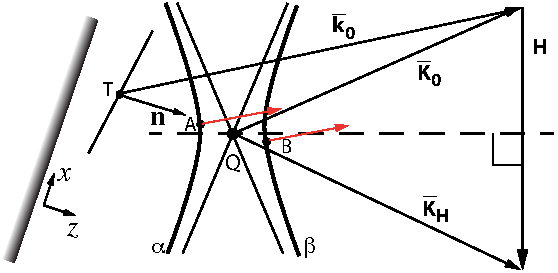
\includegraphics[width=4in]{crystal-energy.pdf}
  \caption[Reference energy flow for Laue diffraction]{
Energy flow used to determine the reference orbit for Laue diffraction.
  }
\label{f:crystal.energy}
\end{figure}

%-------------------------------------------------------------------------
\subsection{Laue Reference Orbit}
\label{s:laue.ref}

For Laue diffraction, with the reference orbit following the \vn{undiffracted} beam, the reference
orbit at the exit surface is just the extension of the reference orbit at the entrance
surface. Since the reference orbit's direction is $\bfkbar_0$.  the reference orbit displacement
vector $\bfL$ (cf.~\Eq{vwlv}) is given by
\Begineq
  \bfL = \frac{t^2}{d\bfkbar_0 \dotproduct \Bf t} \, d\bfkbar_0
  \qquad \text{[undiffracted]}
\Endeq
where
\Begineq
  \Bf t = \begin{pmatrix}
    0 \\ 0 \\ t
  \end{pmatrix}
\Endeq
with $t$ being the crystal thickness and the $z$-axis pointing into the crystal as illustrated in
\fig{f:crystal.energy}. The $\bfS$ roatation matrix (\Eq{wws}) for the undiffracted beam referece
will be the unit matrix.

With the reference orbit following the \vn{forward_diffracted} or \vn{Bragg_diffracted} beam, the
displacement vector $\bfL$ follows the energy flow associated with the tie points labeled $A$ or $B$
in \fig{f:crystal.energy}. These tie points are defined by the intersection of the dispersion
surfaces and the vector $\Bf n$ originating from the point $T$ as shown in the figure.  The energy
flow is perpendicular to the dispersion surface and it can be shown that since, by construction,
$\Bf n$ goes through the $Q$ point, and since the dispersion surfaces are hyperbolies, the energy
flows from $A$ and $B$ tie points are colinear. The direction of the energy flow is given by:
\Begineq
  \bfKbar_f = \xi_H \, \bfKbar_H + \xi_0 \, \bfKbar_0
\Endeq
where $\xi_H$ and $\xi_0$ are given by \cite{b:batterman} Eq.~(18) (See section \sref{s:bragg.track} below).
$\bfL$ is thus
\Begineq
  \bfL = \frac{t^2}{\bfKbar_f \dotproduct \Bf t} \, \bfKbar_f
\Endeq
At the exit surface, if the reference orbit is following the \vn{forward_diffracted} beam, the
orientation of the \vn{element exit} coordinates will be the same as the orientation of the
\vn{element entrance} coordinates. That is, $\bfS$ (\Eq{wws}) is the unit matrix.  If the reference
orbit is following the \vn{Bragg diffracted} beam, $\bfS$ is the same as for Bragg diffraction
\Begineq
  \bfS = 
  \begin{pmatrix}
    \cos\theta_{bend} & 0 & -\sin\theta_{bend} \\
    0                 & 1 & 0           \\
    \sin\theta_{bend} & 0 & \cos\theta_{bend}
  \end{pmatrix}
\Endeq

%-------------------------------------------------------------------------
\subsection{Crystal Surface Reflections and Refractions}

%%%\begin{figure}[tb]
%%%  \centering
%%%  \includegraphics[width=5in]{crystal-surface-reflect.pdf}
%%%  \caption[Reflection from a crystal surface.]
%%%{Reflection from a crystal surface.}
%%%  \label{f:crystal.reflect}
%%%\end{figure}


There are corrections to the field amplitude and phase when a photon reflects or refracts from the
surface of a crystal. A plane wave is incident on a crystal surface with
\Begineq
  E = \what E_0 \, \exp(i \, \bfk_0 \, \bfr)
\Endeq
An outgoing plane wave has a field
\Begineq
  E = \what E_1 \, \exp(i \, \bfk_1 \, \bfr)
\Endeq
A simulation of this condition will start with a number of photons with wave vector $\bfk_0$ and
electric field $E_0$. After reflecting from the surface, the photons will have wave vector
$\bfk_1$. Now imagine a set of $N$ photons that flow through an planar area $dA_0$, perpendicular to
the incoming beam, before being reflected from the surface.

Since the electric field is $\what E_0$, when tracking incoherent photons
\Begineq
  \what E_0^2 = \frac{\alpha_p \, E_0^2 \, N}{dA_0}
\Endeq
where $\alpha_p$ is the simulation constant (cf.~\Eq{panda1}. 
After the photons are reflected they will have some field $E_1$ and thus
\Begineq
  \what E_1^2 = \frac{\alpha_p \, E_1^2 \, N}{dA_1}
\Endeq
Where $dA_1$ is the area that the phtons flow through which is related
to $dA_0$ via
\Begineq
  \frac{dA_1}{dA_0} = \frac{\bfk_1 \cdot \bfz}{\bfk_0 \cdot \bfz} \equiv |b|
\Endeq
Combining the above three equations, the change in field for a photon
as it reflects from the surface is
\Begineq
  \frac{E_1}{E_0} = \frac{\what E_1}{\what E_0} \, \sqrt{|b|} 
  \qquad \text{Incoherent}
\Endeq

For coherent photon tracking the electric field at $dA_0$ is
\Begineq
  \what E_0 = \frac{\alpha_p \, E_0 \, N}{dA_0}
\Endeq
After the photons are reflected they will have some field $E_1$ and thus
\Begineq
  \what E_1 = \frac{\alpha_p \, E_1 \, N}{dA_1}
\Endeq
Combining these equations the change in field for a photon
as it reflects from the surface is
\Begineq
  \frac{E_1}{E_0} = \frac{\what E_1}{\what E_0} \, |b| 
  \qquad \text{Coherent}
\Endeq

Additionally, for coherent tracking, all photons in a plane wave must
have the same phase when passing through an area transverse to the
wave. Thus the two photons labeled $a$ and $b$ in
\fig{f:crystal.reflect} must have the same phase advance in going from
$dA_0$ to $dA_1$. The difference in the phase advance for photon $b$
relative to $a$ from $dA_0$ to the surface is $\bfk_0 \cdot \bfr$
where $\bfr$ is the vector between where photon $b$ hits the surface
relative to phton $a$. Similarly, the difference in the phase advance
for photon $b$ relative to $a$ from the surface to $dA_0$ is $-\bfk_1
\cdot \bfr$. Since the total phase advance for both photons is the
same from $dA_0$ to $dA_1$ the phase shift $d\phi_b$ of photon $b$ as
it is reflected from the surface relative to the phase shift $d\phi_a$
is
\Begineq
  d\phi_b = d\phi_a - (\bfk_1 - \bfk_0) \cdot \bfr
  \label{dpbdpa}
\Endeq

This shift in the reflection phase can be related to the lattice
diffration planes. The wave vector difference can be written
\Begineq
  \bfk_1 - \bfk_0 = \bfH + q \, \bfhat n
  \label{k1k0}
\Endeq
where $\bfhat n$ is perpendicular to the surface. Combining
\Eqs{dpbdpa} and \eq{k1k0} and since $\bfr$ is in
the plane of the surface
\Begineq
  d\phi_b = d\phi_a - \bfH \cdot \bfr
\Endeq
This shows that the reflection shift has the same periodicity as the
pattern of the lattice planes at the surface of the crystal. Notice
that for a mirror, where one point on the surface is the same as any
other, $d\phi_b$ must be equal to $d\phi_a$. Using this in \Eq{dpbdpa}
gives 
\Begineq
  \bfk_1 \cdot \bfr = \bfk_0 \cdot \bfr
\Endeq
and since $|\bfk_1| = |\bfk_0|$ this proves that the angle of
incidence is equal to the angle of reflection for a mirror.

In practice, the registration of the surface planes with respect to
the surface is not specified in a simulation. Thus the reflection
phase shift can only be calculated up to a constant offset. 

%-------------------------------------------------------------------------
\subsection{Bragg Crystal Tracking}
\label{s:bragg.track}

The starting photon coordinates are specified in the laboratory
entrance coordinates. The transformation from laboratory entrance
coordinates to element entrance coordinates $\bftilde k_0$ is given in
\sref{s:photon.lab.ele}. The transformation to element surface
coordinates $\bfk_0$ is
\begin{equation}
  \bfk_0 =  \Bf\Sigma_2 \, \bftilde k_0
\end{equation}
with $\Bf\Sigma_2$ given by \Eq{mt0t010}.
The outgoing wave vector $\bfk_H$ is related to $\bfk_0$ via
\Begineq
  \bfk_H =  \bfk_0 + \bfH + q_t \, \bfhat n
\Endeq
where $q_t$ is determined by using \Eqs{k1lst} and \eq{h1daa} in \Eq{kk1l1}
\begin{align}
  k_{H,x} &= k_{0,x} + H_x \nonumber \CRNO
  k_{H,y} &= k_{0,y} + H_y \\
  k_{H,z} &= \sqrt{\lambda^2 - k_{H,x}^2 - k_{H,y}^2} \nonumber
\end{align}

To compute the field amplitude of the outgoing photon, the equation to
be solved is (\cite{b:batterman} Eq.~(21))
\Begineq
  \xi_0 \, \xi_H = \frac{1}{4} \, k^2 \, P^2 \, \Gamma^2 \, F_H \, F_{\bar H}
  \label{xx14}
\Endeq
where $\xi_0$ and $\xi_H$ are given by \cite{b:batterman} Eq.~(18)
and $P$ is the polarization factor
\Begineq
  P = 
  \begin{cases}
    1               & \sigma \text{ polarization state} \\
    \cos 2\theta_g  & \pi \text{ polarization state}
  \end{cases}
\Endeq
$2\theta_g$ is the angle between $\bfK_0$ and $\bfK_H$ which is well
approximated by $\theta_{B,in} + \theta_{B,out}$.

The solution to \Eq{xx14} is (\cite{b:batterman} Eq.~(31))
\begin{align}
  \xi_0 &= \frac{1}{2} \, k \, |P| \, \Gamma \, [F_H \, F_{\bar H}]^{1/2} \, 
    |b|^{1/2} \, [\eta \pm (\eta^2 + \sign(b))^{1/2}] \CRNO
  \xi_H &= \frac{1}{2} \, k \, |P| \, \Gamma \, [F_H \, F_{\bar H}]^{1/2} \, 
    \frac{1}{|b|^{1/2} \, [\eta \pm (\eta^2 + \sign(b))^{1/2}]}
\end{align}
where the $+$ part of $\pm$ is for the $\alpha$ branch and the $-$
part of $\pm$ is for the $\beta$ branch and $\sign$ is the sign
function
\Begineq
  \sign(b) \equiv \begin{cases} 1 & b > 0 \\ -1 & b < 0 \end{cases}
\Endeq
and $\eta$ is given by \cite{b:blasdell} Eq.~(5)
\Begineq
  \eta = \frac{-b \, a + \Gamma \, F_0 \, (1 - b)}{2 \, \Gamma \, |P| \, \sqrt{|b| \, F_H \, F_{\bar H}}}
\Endeq
with the asymmetry factor $b$ for the photon being tracked being given
by \cite{b:blasdell} Eq.~(3)
\Begineq
  b \equiv \frac{\bfhat n \dotproduct \bfhat k_0}{\bfhat n \dotproduct (\widehat{{\bfk_0 + \bfH}})}
\Endeq
and the angular deviation variable $a$ is given by \cite{b:blasdell} Eq.~(4)
\Begineq
  a \equiv \frac{H^2 + 2 \, \bfk_0 \dotproduct \bfH}{k_0^2} 
  = -2 \, \Delta \theta \, \sin(2\theta_B)
\Endeq
Once $\xi_0$ and $\xi_H$ are determined, the ratio of the incoming and outgoing fields
for the $\alpha$ or $\beta$ branches can be computed via (\cite{b:batterman} Eq.~(24))
\Begineq
  r_E \equiv \frac{\bfE_H}{\bfE_0} 
  = \frac{- \, 2 \, \xi_0}{k \, P \, \Gamma \, F_{\bar H}} \,
  = \, \frac{- \, k \, P \, \Gamma \, F_H}{2 \, \xi_H} 
\Endeq
where the $\alpha$ or $\beta$ subscript has been supressed.  The total
field which is the sum of the fields on the branches is computed using
the boundary conditions
\Begineq
  \bfE_0 = \bfE_{0\alpha} + \bfE_{0\beta}, \qquad\qquad 
  0 = \bfE_{H\alpha} + \bfE_{H\beta}
\Endeq
Using the above two equations gives
\begin{align}
  \bfE_{0\alpha} &= \bfE_0 \, \frac{r_{E\beta}}{r_{E\beta} - r_{E\alpha}} \qquad\qquad
  \bfE_{H\alpha}  = \bfE_0 \, \frac{r_{E\alpha} \, r_{E\beta}}{r_{E\beta} - r_{E\alpha}} \CRNO
  \bfE_{0\beta} &= -\bfE_0 \, \frac{r_{E\alpha}}{r_{E\beta} - r_{E\alpha}} \qquad\qquad
  \bfE_{H\beta}  = -\bfE_0 \, \frac{r_{E\alpha} \, r_{E\beta}}{r_{E\beta} - r_{E\alpha}} 
\end{align}

As can be seen from Battermann and Cole Figs.~(8) and (29), the
$\alpha$ tie point is excited and the $\beta$ tie point is not if
$\xi_{0\alpha} < \xi_{0\beta}$ and vice versa. Since only one tie
point is excited, The external field ratio is equal to
the internal field ratio 
\Begineq
  \frac{E_H^e}{E_0^i} = \frac{E_{Hj}}{E_{0j}}
\Endeq
where $j$ is $\alpha$ or $\beta$ as appropriate.

%-------------------------------------------------------------------------
\subsection{Coherent Laue Crystal Tracking}
\label{s:coherent.laue}

Laue diffraction has two interior wave fields (branches), labeled
$\alpha$ and $\beta$, corresponding to the two tie points that are
excited on the two dispersion surfaces. For coherent tracking, a
photon has some probability to be channeled to follow the $\alpha$ or
$\beta$ branch. The electric field ratios $\what E_\alpha$ and $\what
E_\beta$ (cf.~\Eq{rpss2}) are taken to be equal to each other. With
this choice, the probabilities $P_\alpha$ and $P_\beta$ for being
channeled to the $\alpha$ or $\beta$ branches are such that a branch
with a greater intensity will have a greater number of photons
chanelled down it.

When a crystal's \vn{ref_orbit_follows} parameter is set to
\vn{bragg_diffracted}, The branching probabilities are
\Begineq
  P_\alpha = \frac{|E_{H\alpha}|}{|E_{H\alpha}| + |E_{H\beta}|} , \qquad
  P_\beta = \frac{|E_{H\beta}|}{|E_{H\alpha}| + |E_{H\beta}|} , \qquad
  \what E_{H\alpha} = \what E_{H\beta}  = \frac{|E_{H\alpha}| + |E_{H\beta}|}{|E_0^i|}
\Endeq
where (see Batermann and Cole\cite{b:batterman} Eqs~(42)), 
\begin{align}
  E_{H\alpha} &= -E_0^i \, \dsfrac{|b|^{1/2}}{2 \, \cosh v} \, 
    \frac{|P|}{P} \, 
    \frac{[F_H \, F_\Hbar]^{1/2}}{F_H} \, 
    \exp({-2 \, \pi \, i \, \bfK'_{H\alpha} \dotproduct \bfr_\alpha}) \,
    \exp({-2 \, \pi \, \bfK''_{H\alpha} \dotproduct \bfr_\alpha}) \CRNO
  E_{H\beta} &= E_0^i \, \dsfrac{|b|^{1/2}}{2 \, \cosh v} \, 
    \frac{|P|}{P} \, 
    \frac{[F_H \, F_\Hbar]^{1/2}}{F_H} \, 
    \exp({-2 \, \pi \, i \, \bfK'_{H\beta} \dotproduct \bfr_\beta}) \,
    \exp({-2 \, \pi \, \bfK''_{H\beta} \dotproduct \bfr_\beta})
\end{align}
where $\bfr_\alpha$ and $\bfr_\beta$ are the vectors from the
entrance surface to the exit surface for the $\alpha$ and $\beta$ wave
fields
\Begineq
  \bfr_\alpha = \frac{t^2}{\bfS_\alpha \dotproduct \Bf t} \, \bfS_\alpha , \qquad
  \bfr_\beta = \frac{t^2}{\bfS_\beta \dotproduct \Bf t} \, \bfS_\beta
\Endeq
with
\begin{align}
  \bfS_\alpha &= e^{-2 \, v} \, \Bf s_0 + \left| b \, \frac{F_H \, F_\Hbar}{F_H^2} \right| \, \Bf s_H \CRNO
  \bfS_\beta &= e^{2 \, v} \, \Bf s_0 + \left| b \, \frac{F_H \, F_\Hbar}{F_H^2} \right| \, \Bf s_H 
\end{align}
The phase shift of the electric field is obtained from the phase of
$E_{H\alpha}$ if the photon is channeled into the $\alpha$ branch and
$E_{H\beta}$ if the photon is channeled into the $\beta$ branch.

When a crystal's \vn{ref_orbit_follows} parameter is set to
\vn{forward_diffracted} or \vn{undefracted}, the algorithm is similar
to the \vn{bragg_diffracted} case except $E_{0\alpha}$ and
$E_{0\beta}$ are used in place of $E_{H\alpha}$ and
$E_{H\beta}$ with
\begin{align}
  E_{0\alpha} &= E_0^i \, \dsfrac{e^{-v}}{2 \, \cosh v} \, 
    \exp({-2 \, \pi \, i \, \bfK'_{0\alpha} \dotproduct \bfr_\alpha}) \,
    \exp({-2 \, \pi \, \bfK''_{0\alpha} \dotproduct \bfr_\alpha}) \CRNO
  E_{0\beta} &= E_0^i \, \dsfrac{e^{-v}}{2 \, \cosh v} \, 
    \exp({-2 \, \pi \, i \, \bfK'_{0\beta} \dotproduct \bfr_\alpha}) \,
    \exp({-2 \, \pi \, \bfK''_{0\beta} \dotproduct \bfr_\beta})
\end{align}

Since a simulation photon has two polarization components, the above
equations are used for one polarization component and for the second
polarization component the same branch is used as for the first with
an appropriately scaled $\what E$.

%-------------------------------------------------------------------------
\subsection{Incoherent Laue Crystal Tracking}
\label{s:incoherent.laue}

Laue diffraction has two interior wave fields (branches), labeled
$\alpha$ and $\beta$, corresponding to the two tie points that are
excited on the two dispersion surfaces. For incoherent tracking it is
assumed that these wave fields overlap at the exit surface
(\cite{b:batterman} Eq.~(87)) and so add coherently. This is a good
approximation if the crystal is very thin where the wave fields do not
travel an appreciable spatial distance and is also a good
approximation when the crystal is thick since the $\beta$ branch will
be heavily attenuated. At intermediate thicknesses this approximation
is good when a photon is near the Bragg angle since, in this case, the
fields will be traveling in similar directions.

Another approximation is that the path

\begin{align}
  E_{H\alpha} &= -E_0^i \, \dsfrac{|b|^{1/2}}{2 \, \cosh v} \, 
    \frac{|P|}{P} \, 
    \frac{[F_H \, F_\Hbar]^{1/2}}{F_H} \, 
    \exp({-2 \, \pi \, i \, \bfK'_{H\alpha} \dotproduct \bfr_\alpha}) \,
    \exp({-2 \, \pi \, \bfK''_{H\alpha} \dotproduct \bfr_\alpha}) \CRNO
  E_{H\beta} &= E_0^i \, \dsfrac{|b|^{1/2}}{2 \, \cosh v} \, 
    \frac{|P|}{P} \, 
    \frac{[F_H \, F_\Hbar]^{1/2}}{F_H} \, 
    \exp({-2 \, \pi \, i \, \bfK'_{H\beta} \dotproduct \bfr_\beta}) \,
    \exp({-2 \, \pi \, \bfK''_{H\beta} \dotproduct \bfr_\beta})
\end{align}


%-------------------------------------------------------------------------
\section{X-ray Targeting}
\label{s:targeting}

X-rays can have a wide spread of trajectories resulting in many
``doomed'' photons that hit apertures or miss the detector with only a
small fraction of ``successful'' photons actually contributing to the
simulation results. The tracking of doomed photons can therefore
result in an appreciable lengthening of the simulation time. To get
around this, \bmad can be setup to use what is called ``targeting'' to
greatly reduce the number of doomed photons generated.

Photons can be generated either at a source like a \vn{wiggler}
element or at a place where diffraction is simulated like at a
\vn{diffraction_plate} element. To be able to do targeting, an element
with apertures defined must be present downstream from the generating
element. The idea is to only generate photons that are going in the
general direction of the ``target'' which is the space within the
aperture.

A necessary restriction for
targeting to work is that the photon must travel in a straight line
through all elements between the generating element and the element
with the apertures. So, for example, a \vn{crystal} element would not
be allowed between the two two elements. A \vn{crystal} element could
be the aperture element as long as the aperture was defined before
photons were diffracted. That is, if the aperture was at the upstream
end of the crystal or was defined with respect to the \vn{crystal}
surface.

The target is defined by the four corners of the aperture. In \vn{element}
coordinates, the $(x, y, z)$ values of the corners are:
\begin{example}
  (-x1_limit, -y1_limit, z_lim)
  (-x1_limit,  y2_limit, z_lim)
  ( x2_limit, -y1_limit, z_lim)
  ( x2_limit,  y2_limit, z_lim)
\end{example}
where \vn{x1_limit}, etc. are the aperture limits (\sref{s:limit})
and \vn{z_lim} will be zero except if the element's \vn{aperture_at}
parameter is set to \vn{entrance_end} in which case \vn{z_lim} will be set
to \vn{-L} where \vn{L} is the length of the element. 

If the aperture is associated with a curved surface (for example with
a \vn{crystal} element), four extra corner points are also used to
take into account that the aperture is not planar. These extra points
have $(x, y, z)$ values in \vn{element} coordinates of
\begin{example}
  (-x1_limit, -y1_limit, z_surface(-x1_limit, -y1_limit))
  (-x1_limit,  y2_limit, z_surface(-x1_limit,  y2_limit))
  ( x2_limit, -y1_limit, z_surface( x2_limit, -y1_limit))
  ( x2_limit,  y2_limit, z_surface( x2_limit,  y2_limit))
\end{example}
where \vn{z_surface(x,y)} is the $z$ value of the surface at the
particular $(x, y)$ point being used. Notice that in this case
\vn{z_lim} is zero.

The coordinates of the four or eight corner points are converted from
\vn{element} coordinates of the aperture element to \vn{element}
coordinates of the photon generating element. Additionally,
the approximate center of the aperture, which in \vn{element}
coordinates of the aperture element is $(0, 0, z_lim)$, is converted
to \vn{element} coordinates of the photon generating element.

The above calculation only has to be done once at the beginning of a
simulation.

When a photon is to be emitted from a given point $(x_{emit},
y_{emit}, z_{emit})$, the problem is how to restrict the velocity
vector $(\beta_x, \beta_y, \beta_z)$ (which is normalized to 1) to
minimize the number of doomed photons generated. The problem is solved
by constructing a vector $\Bf r$ for each corner point:
\Begineq
  \Bf r = (x_{lim}, y_{lim}, z_{lim}) - (x_{emit}, y_{emit}, z_{emit})
\Endeq 
The direction of each $\Bf r$ is characterized in polar coordinates
$(\phi, y)$ defined by
\begin{align}
  y &= \frac{r_y}{|r|} \CRNO
  \tan\phi &= \frac{r_x}{r_z} 
\end{align}
For now make the assumption that $r_z$ is positive and larger than
$r_x$ and $r_y$ for all $\Bf r$.  Let $\phi_{max}$ and $\phi_{min}$ be
the maximum and minimum $\phi$ values over all the $\Bf r$. Similarly,
let $y_{min}$ and $y_{max}$ be the minimum and maximum $y$ values over
all the $\Bf r$. The rectangle in $(\phi, y)$ space defined by these
four min and max values almost covers the projection of the aperture
onto the unit sphere. There is a correction that must be made due to
the fact that a straight line of constant $y$ in $(x, y, z)$ space
projects to a curved line when projected onto $(\phi, y)$
space. Therefore a correction must be made to $y_{min}$ when $y_{min}
< 0$:
\Begineq
  y_{min} \rightarrow 
  \frac{y_min}{\sqrt{(1 - y_{min}^2) \, \cos^2 (phi_{max} - \phi_{min})/2 + y_{min}^2}}
\Endeq
with a similar correction for $y_{max}$ that must be made when $y_{max} > 0$.


The above prescription works as long as the projection of the aperture
onto $(\phi, y)$ space does not touch the branch cut at $\phi = \pi$
or cover the singular points $y = \pm 1$. Generally these restrictions
are fullfilled since $\Bf z$ is the direction of the reference
orbit. If this is not the case, a transformation can be made where
rotation matrices are constructed to transform between the
\vn{element} coordinates of the emitting element and what are called
\vn{target} coordinates defined so that $\Bf r$ for the \vn{center} point
has the form $(0, 0, |r|)$. The procedure for calculating the photon
velocity vector is now
  \begin{enumerate}
  \item
Rotate all the corner $\Bf r$ from \vn{element} to \vn{target} coordinates.
  \item
Calculate min and max values for $\phi$ and $y$.
  \item
Calculate the velocity vector such that the $(\phi, y)$ of this vector
falls within the min and max values in the last step.
  \item
Rotate the velocity vector back to \vn{element} coordinates.
  \end{enumerate}

